%---------------
% Question 6
%---------------
\begin{problem}{2-6}
Figure \ref{fig:question6_prompt_fig} shows a rocket that is to be approximated
by a particle of instantaneous mass $m(t)$. The instantaneous velocity is $v(t)$,
$T(t)$ is the thrust, and $\beta(t)$ is the thrust angle. If we assume no
aerodynamic drag or gravitational forces, and if we select $x_1 \triangleq x$,
$x_2 \triangleq \dot{x}$, $x_3 \triangleq y$, $x_4 \triangleq \dot{y}$, $x_5 \triangleq m$,
$u_1 \triangleq T$, $u_2 \triangleq \beta$, the state equations are

\begin{align}
  \dot{x_1}(t) &= x_2(t) \nonumber \\
  \dot{x_2}(t) &= \frac{[u_1(t)\, \cos u_2(t)]}{x_5(t)} \nonumber \\
  \dot{x_3}(t) &= x_4(t) \nonumber \\
  \dot{x_4}(t) &= \frac{[u_1(t)\, \sin u_2(t)]}{x_5(t)} \nonumber \\
  \dot{x_5}(t) &= -\frac{1}{c}u_1(t), \nonumber
\end{align}

\noindent where $c$ is a constant of proportionality. The rocket starts from
rest at the point $x = 0$, $y = 0$.
\end{problem}


\begin{figure}[H]
    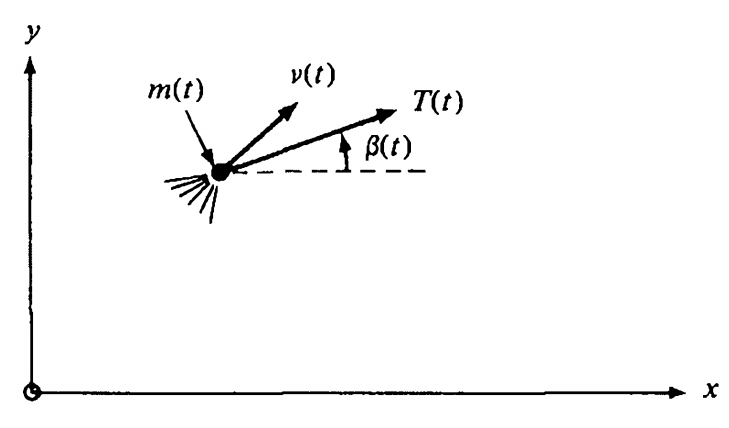
\includegraphics[scale=0.35]{question6_prompt_fig}
    \centering
    \caption{Rocket to be approximated by a particle of instantaneous mass \cite{kirkdover}}
    \label{fig:question6_prompt_fig}
\end{figure}

\noindent \textbf{a)}

A set of physically reasonable \textit{state constraints} are

\begin{align}
  0 &\leq x_1(t) \nonumber \\
  0 &< x_5(t) \nonumber \\
  \int_{t_0}^{t_f} \dot{x_5}&(t) \, dt \leq F_t \nonumber
\end{align}

\noindent where $F_t$ is the total fuel. A set of physically reasonable
\textit{control constraints} are

\begin{align}
     0 \leq & u_1(t) \leq T_{max} \nonumber \\
  -\pi \leq & u_2(t) \leq \pi \nonumber
\end{align}

\noindent where $T_{max}$ is the maximum thrust. The control constraint on $u_2(t)$
stems from the fact that if the rocket were to go beyond these angles ($\pm \pi$)
then the rocket could potentially be pointed towards the earth.

\noindent \textbf{b)}
The objective is to have $y(t_f) = 3$ mi and to maximize $x(t_f)$. A new
physical constraint is

\begin{equation}
  x_3(t_f) = 3 \, \text{mi} \nonumber
\end{equation}

A performance measure for this situation is

\begin{equation}
  J = -x_1^2(t_f) \nonumber
\end{equation}

\noindent A minus sign is used here because this is a \textit{maximization}
problem. Otherwise, the performance measure would cause $x_1(t_f)$ to be
minimized.

\noindent \textbf{c)}
The objective is to have the rocket reach $x = 500$ mi and $y = 3$ mi within
2.5 min with maximum possible vehicle mass.

A set of constraints for this objective is

\begin{align}
  x_1(t_f) &= 500 \text{mi} \nonumber \\
  x_3(t_f) &= 3 \text{mi} \nonumber
\end{align}

A performance measure for this objective is

\begin{equation} \label{eq:q6c_perf_meas}
  J = - q x_5(t_f), \quad q \in \mathbb{R}, \, \text{and} \, q > 0
\end{equation}

\noindent where $q$ is a weight. Equation \ref{eq:q6c_perf_meas} does not
need an absolute value operator or to be squared because the state $x_5$
represents \textit{mass} which can never, as far as it is currently known, be
negative.
